\documentclass{article}
\usepackage[dutch]{babel}
\usepackage{hyperref}
\usepackage{graphicx}
\usepackage[bottom=2.5cm, right=2.5cm, left=2.5cm, top=2.5cm]{geometry}

\title{Eindvergadering ML sessie 08}
\author{Team $\exists$uler\\
	\textit{Daan, Marie, Zeineb, Florian, Vincent, Jasper, Lasha, Younes}}
\date{Vrijdag \today}

\begin{document}
	
\maketitle

\section*{Reflectie}

Deze sessie hebben we onze tekst geherstructureerd, het besluit afgewerkt en zijn we bovendien begonnen aan het ontwerp van onze poster. In figuur \ref{fig:inhoudsopgave} is de zien hoe de opbouw van ons eindverslag dramatisch is veranderd.

\begin{figure}[h!]
	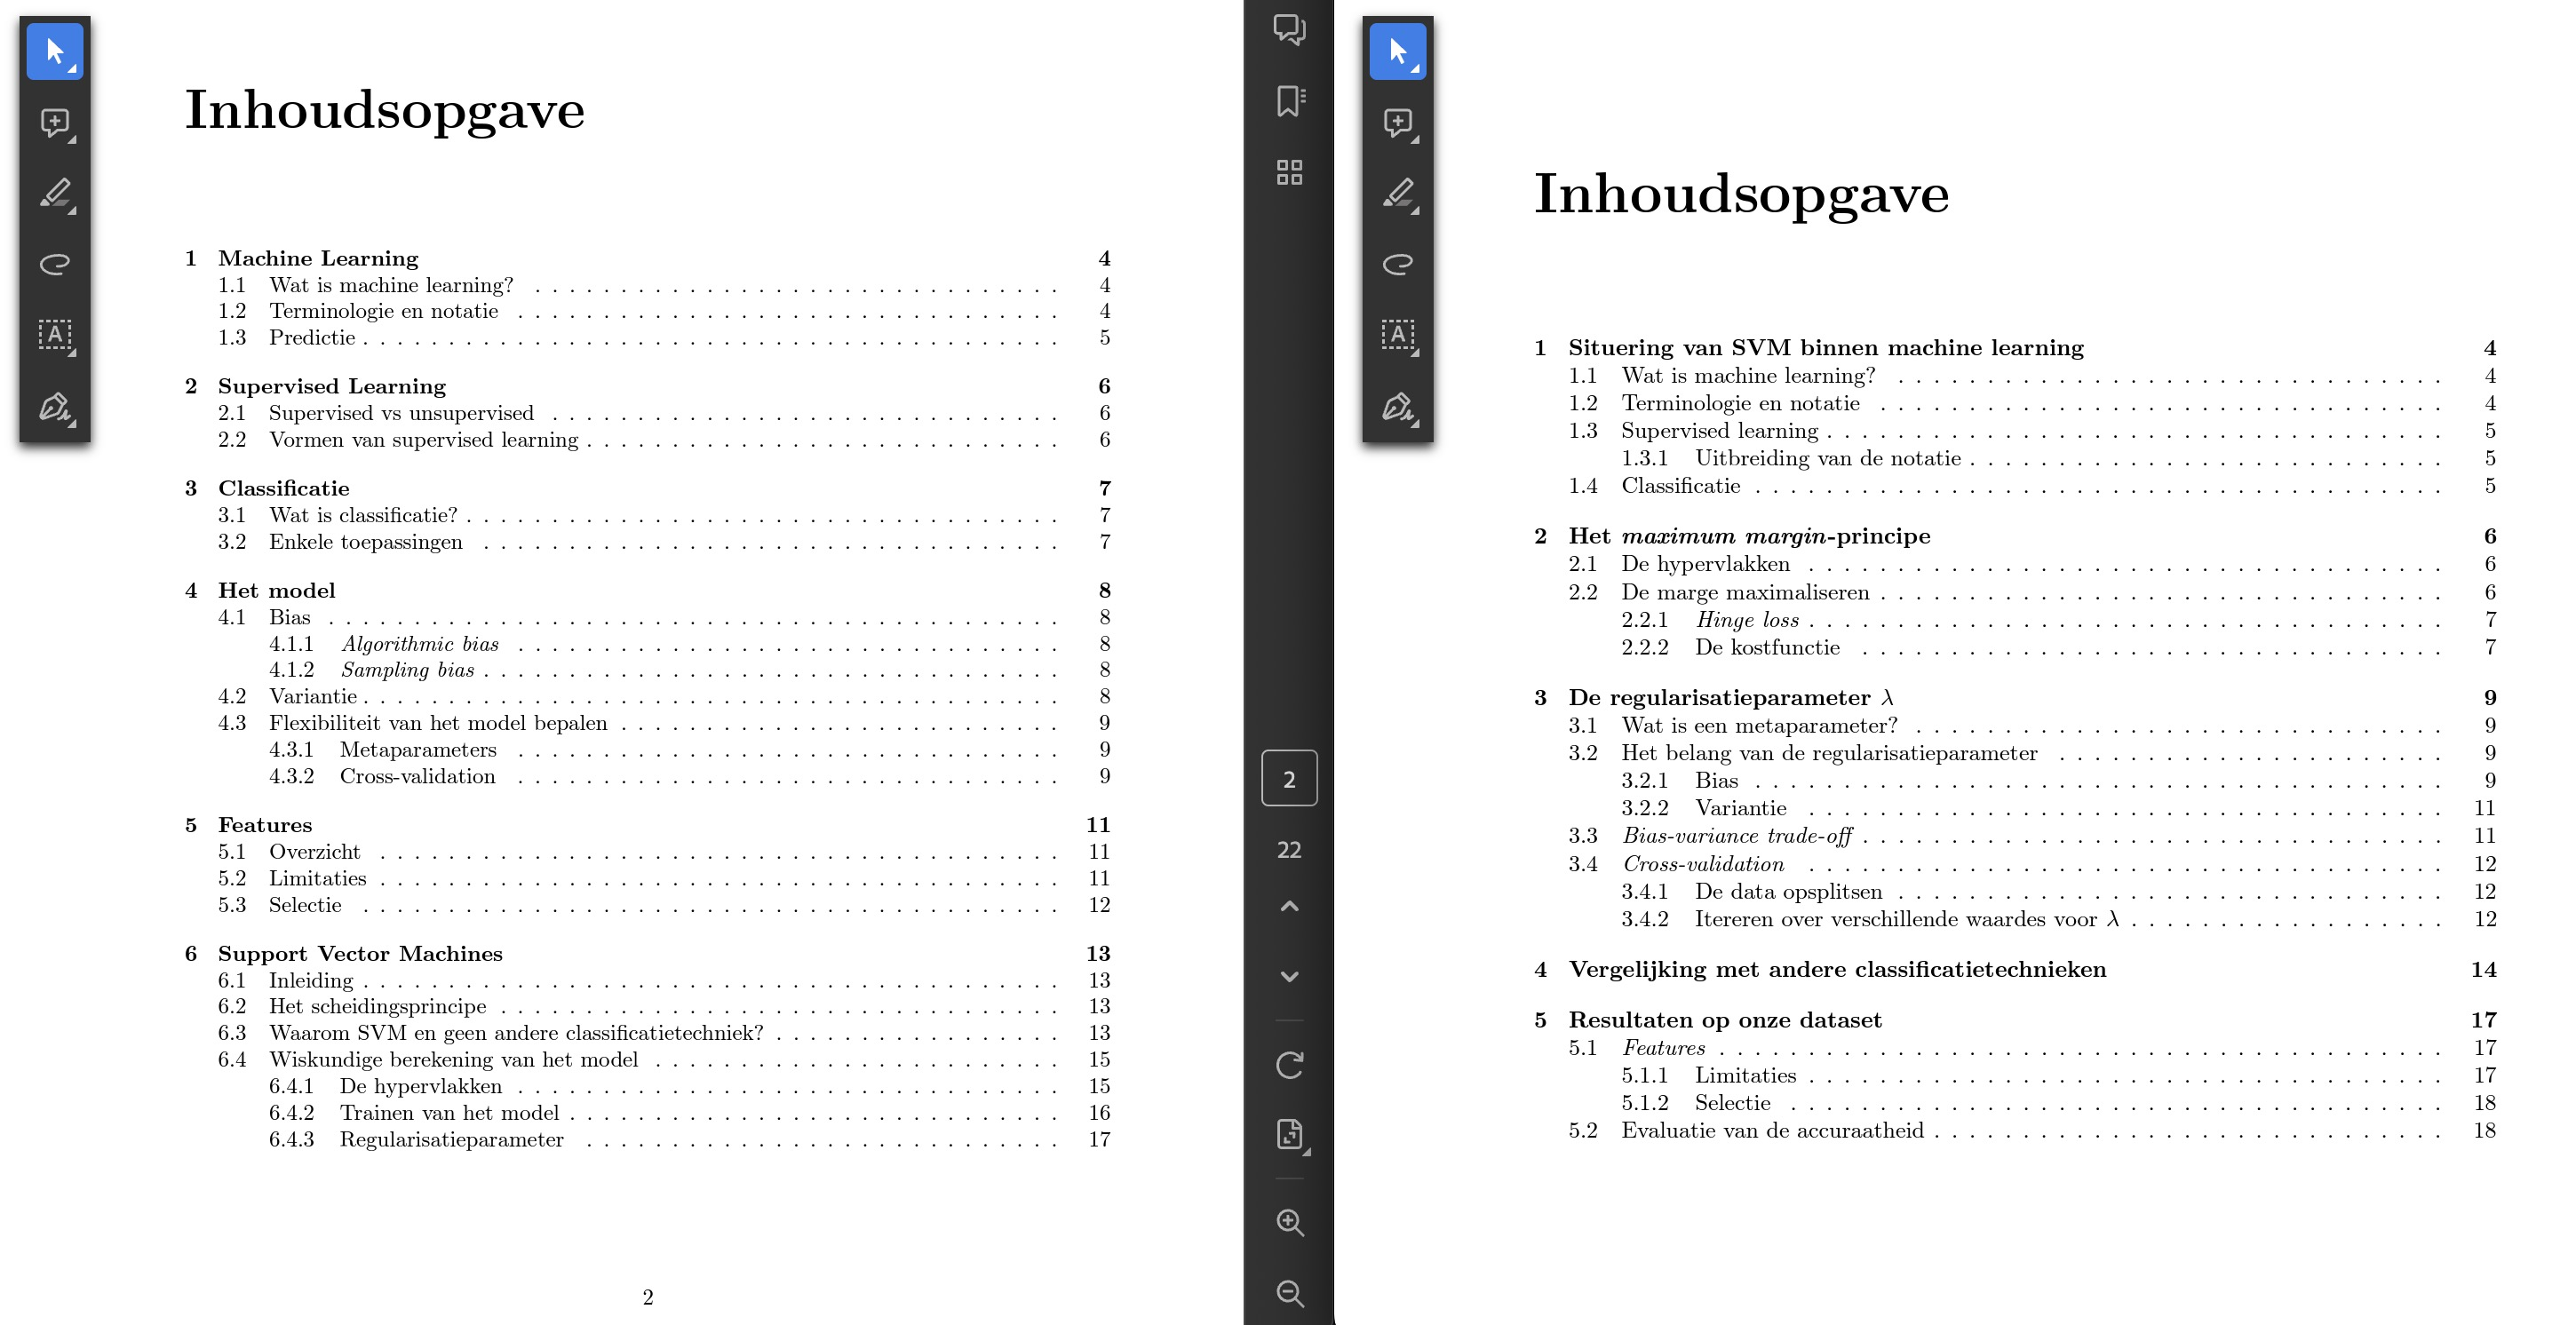
\includegraphics[width=.99\textwidth]{inhoudsopgave}
	\caption{Links is de inhoudsopgave te zien die we hadden vóór sessie 08, rechts staat de inhoudsopgave die we hebben na de complete herwerking van de tekststructuur.}
	\label{fig:inhoudsopgave}
\end{figure}

\end{document}